%%%%%%%%%%%%%%%%%%%%%%%%%%%%%%%%%%%%%%%%%
% Developer CV
% LaTeX Template
% Version 1.0 (28/1/19)
%
% This template originates from:
% http://www.LaTeXTemplates.com
%
% Authors:
% Jan Vorisek (jan@vorisek.me)
% Based on a template by Jan Küster (info@jankuester.com)
% Modified for LaTeX Templates by Vel (vel@LaTeXTemplates.com)
%
% License:
% The MIT License (see included LICENSE file)
%
%%%%%%%%%%%%%%%%%%%%%%%%%%%%%%%%%%%%%%%%%

%----------------------------------------------------------------------------------------
%	PACKAGES AND OTHER DOCUMENT CONFIGURATIONS
%----------------------------------------------------------------------------------------

\documentclass[9pt]{developercv_mattia} % Default font size, values from 8-12pt are recommended
\usepackage{graphicx}
% \usepackage[UKenglish]{babel}
\usepackage[british]{babel}


\tolerance=1
\emergencystretch=\maxdimen
\hyphenpenalty=10000
\hbadness=10000

%----------------------------------------------------------------------------------------

\begin{document}

%----------------------------------------------------------------------------------------
%	TITLE AND CONTACT INFORMATION
%----------------------------------------------------------------------------------------

\begin{minipage}[t]{0.4\textwidth} % 45% of the page width for name
	\vspace{-\baselineskip} % Required for vertically aligning minipages
	
	% If your name is very short, use just one of the lines below
	% If your name is very long, reduce the font size or make the minipage wider and reduce the others proportionately
	% \colorbox{black}{{\HUGE\textcolor{white}{\textbf{\MakeUppercase{Mattia}}}}} % First name
	
	% \colorbox{black}{{\HUGE\textcolor{white}{\textbf{\MakeUppercase{Piazza}}}}} % Last name
	\colorbox{white}{{\HUGE\textcolor{black}{\textbf{\MakeUppercase{Mattia}}}}} % First name
	
	\colorbox{white}{{\HUGE\textcolor{black}{\textbf{\MakeUppercase{Piazza}}}}} % Last name

	\vspace{6pt}
	
	{\huge Researcher\\ Mechatronics Engineer} % Career or current job title
\end{minipage}
\hfill
\begin{minipage}[t]{0.3\textwidth} % 27.5% of the page width for the first row of icons
	\vspace{-\baselineskip} % Required for vertically aligning minipages
	% The first parameter is the FontAwesome icon name, the second is the box size and the third is the text
	% Other icons can be found by referring to fontawesome.pdf (supplied with the template) and using the word after \fa in the command for the icon you want
	\icon{MapMarker}{10}{Trento, TN, Italy}\\
	\icon{Globe}{10}{Italian}\\
	\icon{Phone}{10}{+39 333 15 14 344}\\
	%\icon{At}{10}{\href{mailto:piazzamattia1994@gmail.com}{piazzamattia1994@gmail.com}}\\
	\icon{At}{10}{\href{mailto:mattia.piazza@alumni.unitn.it}{mattia.piazza@unitn.it}}\\
	\icon{Linkedin}{10}{\href{https://www.linkedin.com/in/mattiapiazza/}{mattiapiazza}}\\
	\icon{Github}{10}{\href{https://github.com/Mattiapzz}{Mattiapzz}}\\
	% \icon{\faGitSquare}{10}{Mattiapzz}
	%\icon{Skype}{10}{live:piazzamattia1994}\\
\end{minipage}
\hfill
\begin{minipage}[t]{0.20\textwidth} % 27.5% of the page width for the second row of icons
	\vspace{-\baselineskip} % Required for vertically aligning minipages
		\hfill
	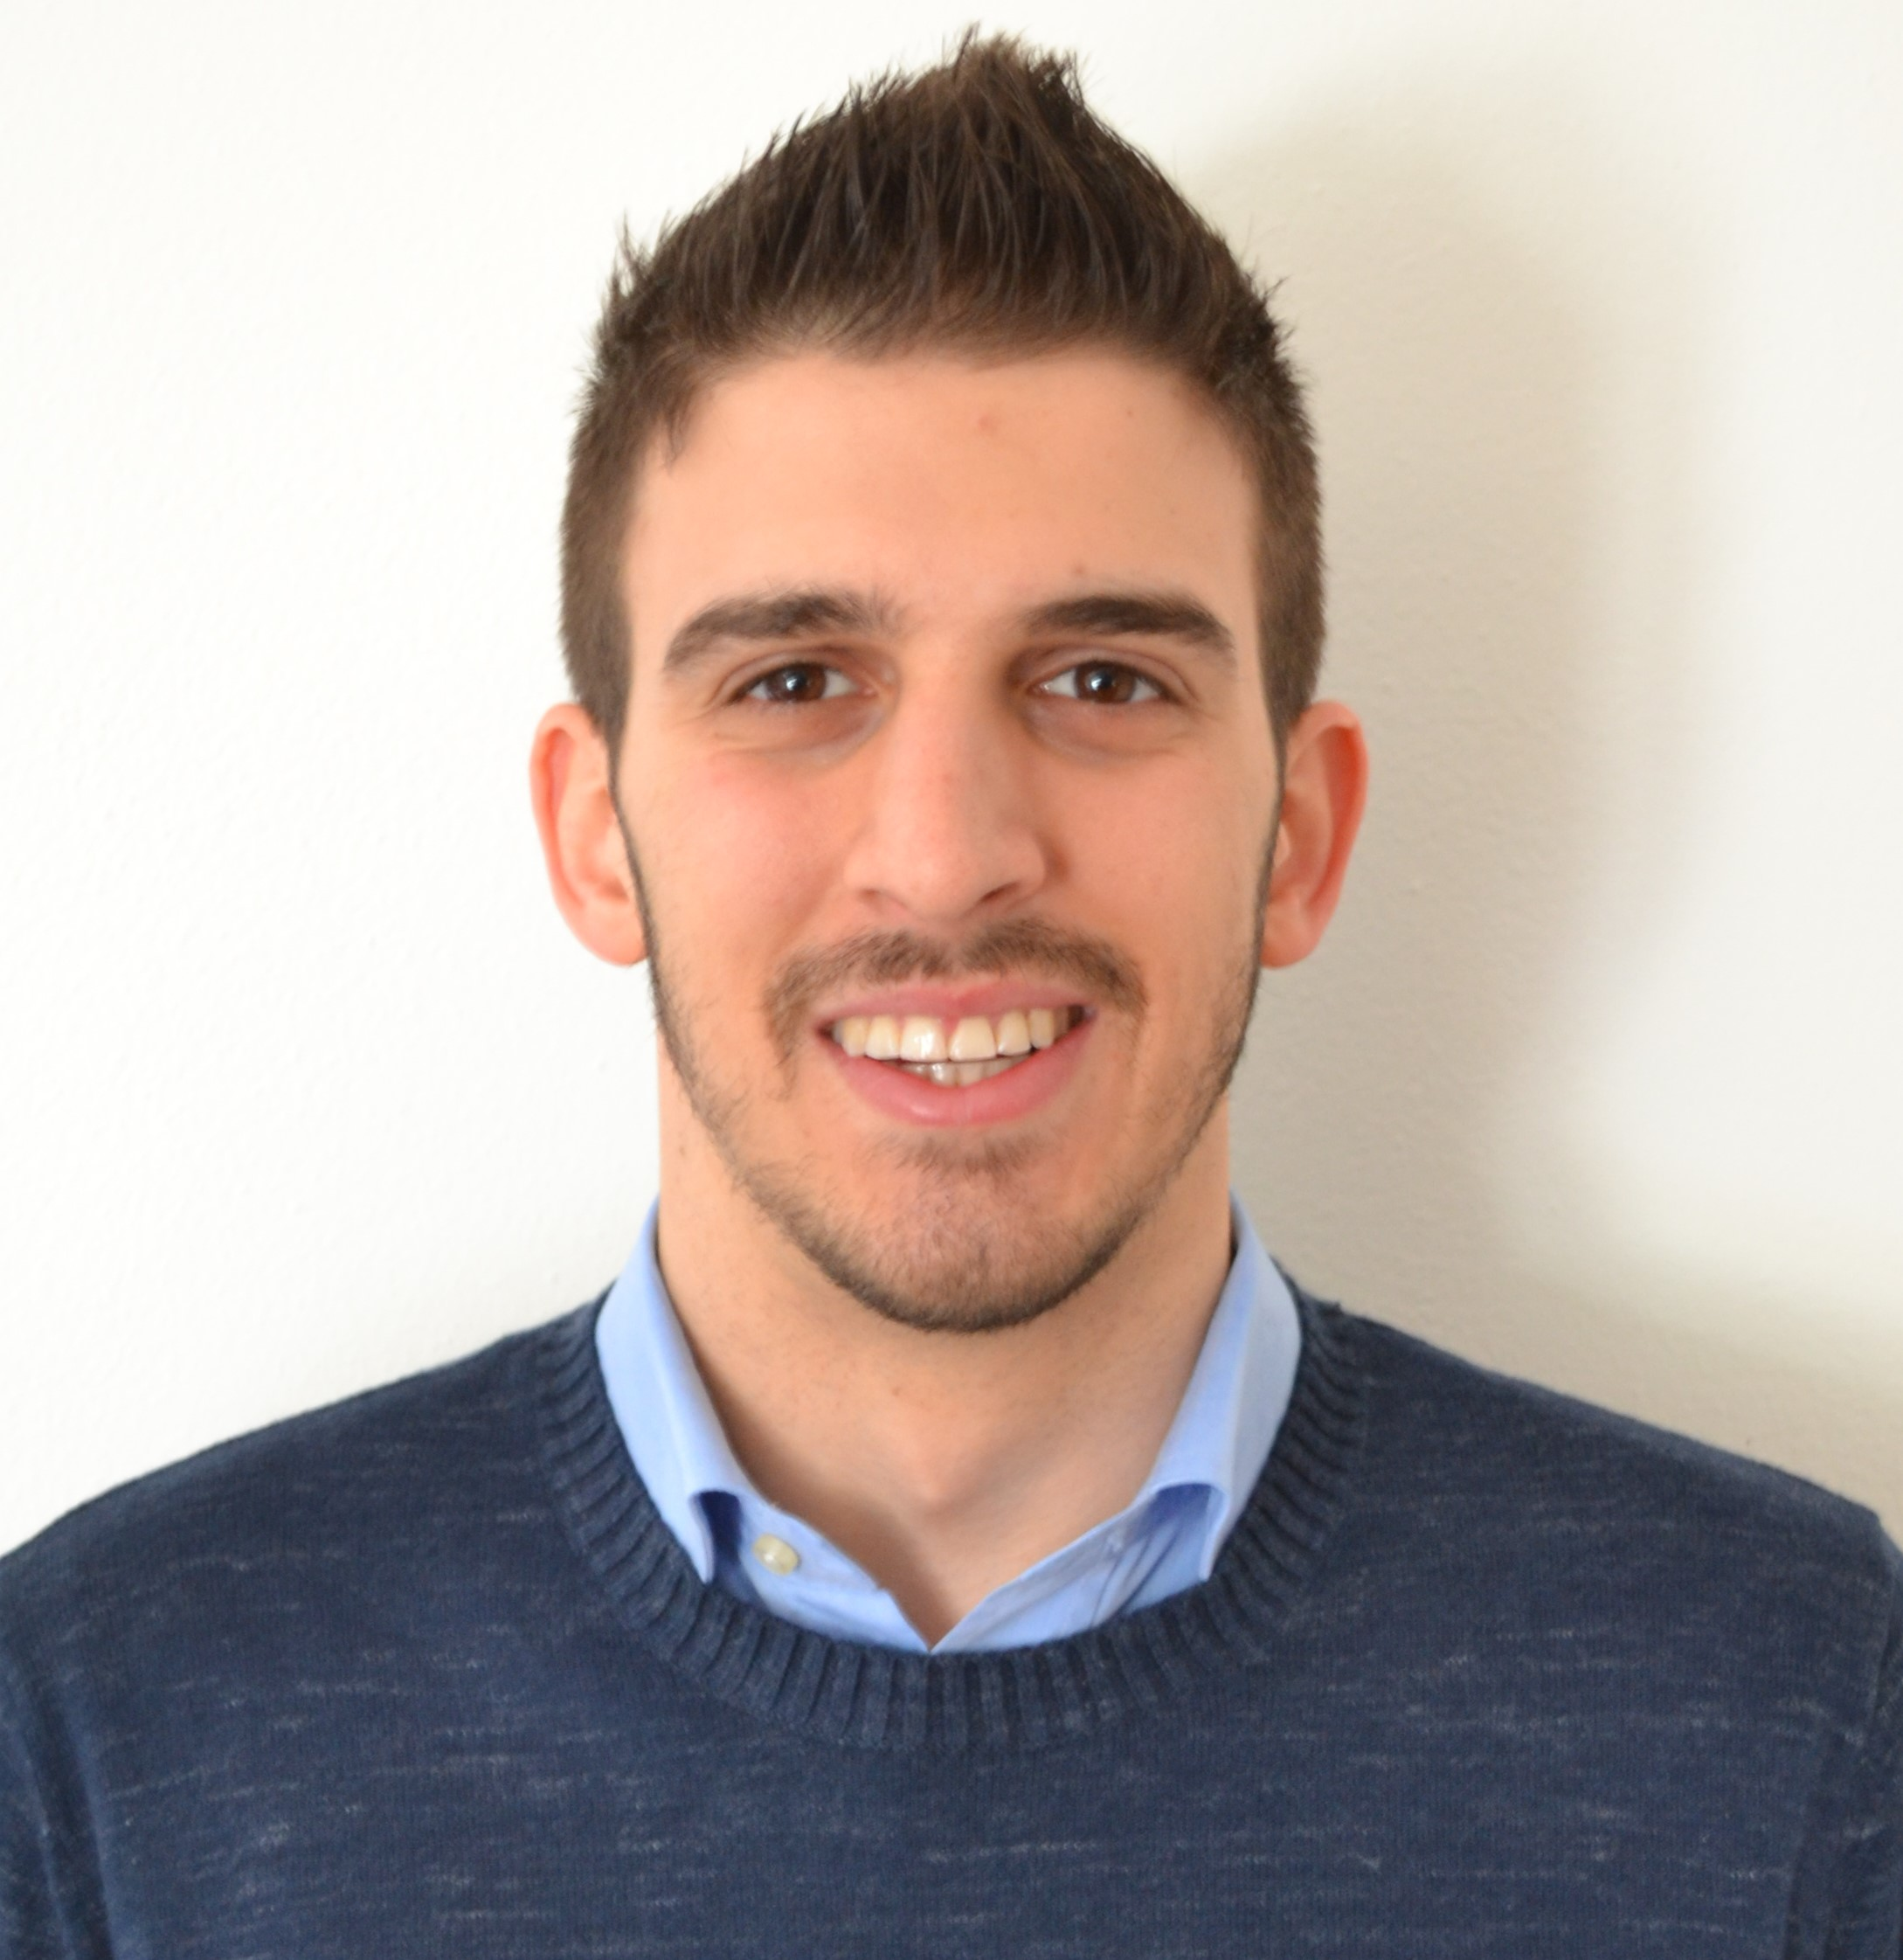
\includegraphics[width=1.0\linewidth]{../shared/Fototessera.jpg}
	% 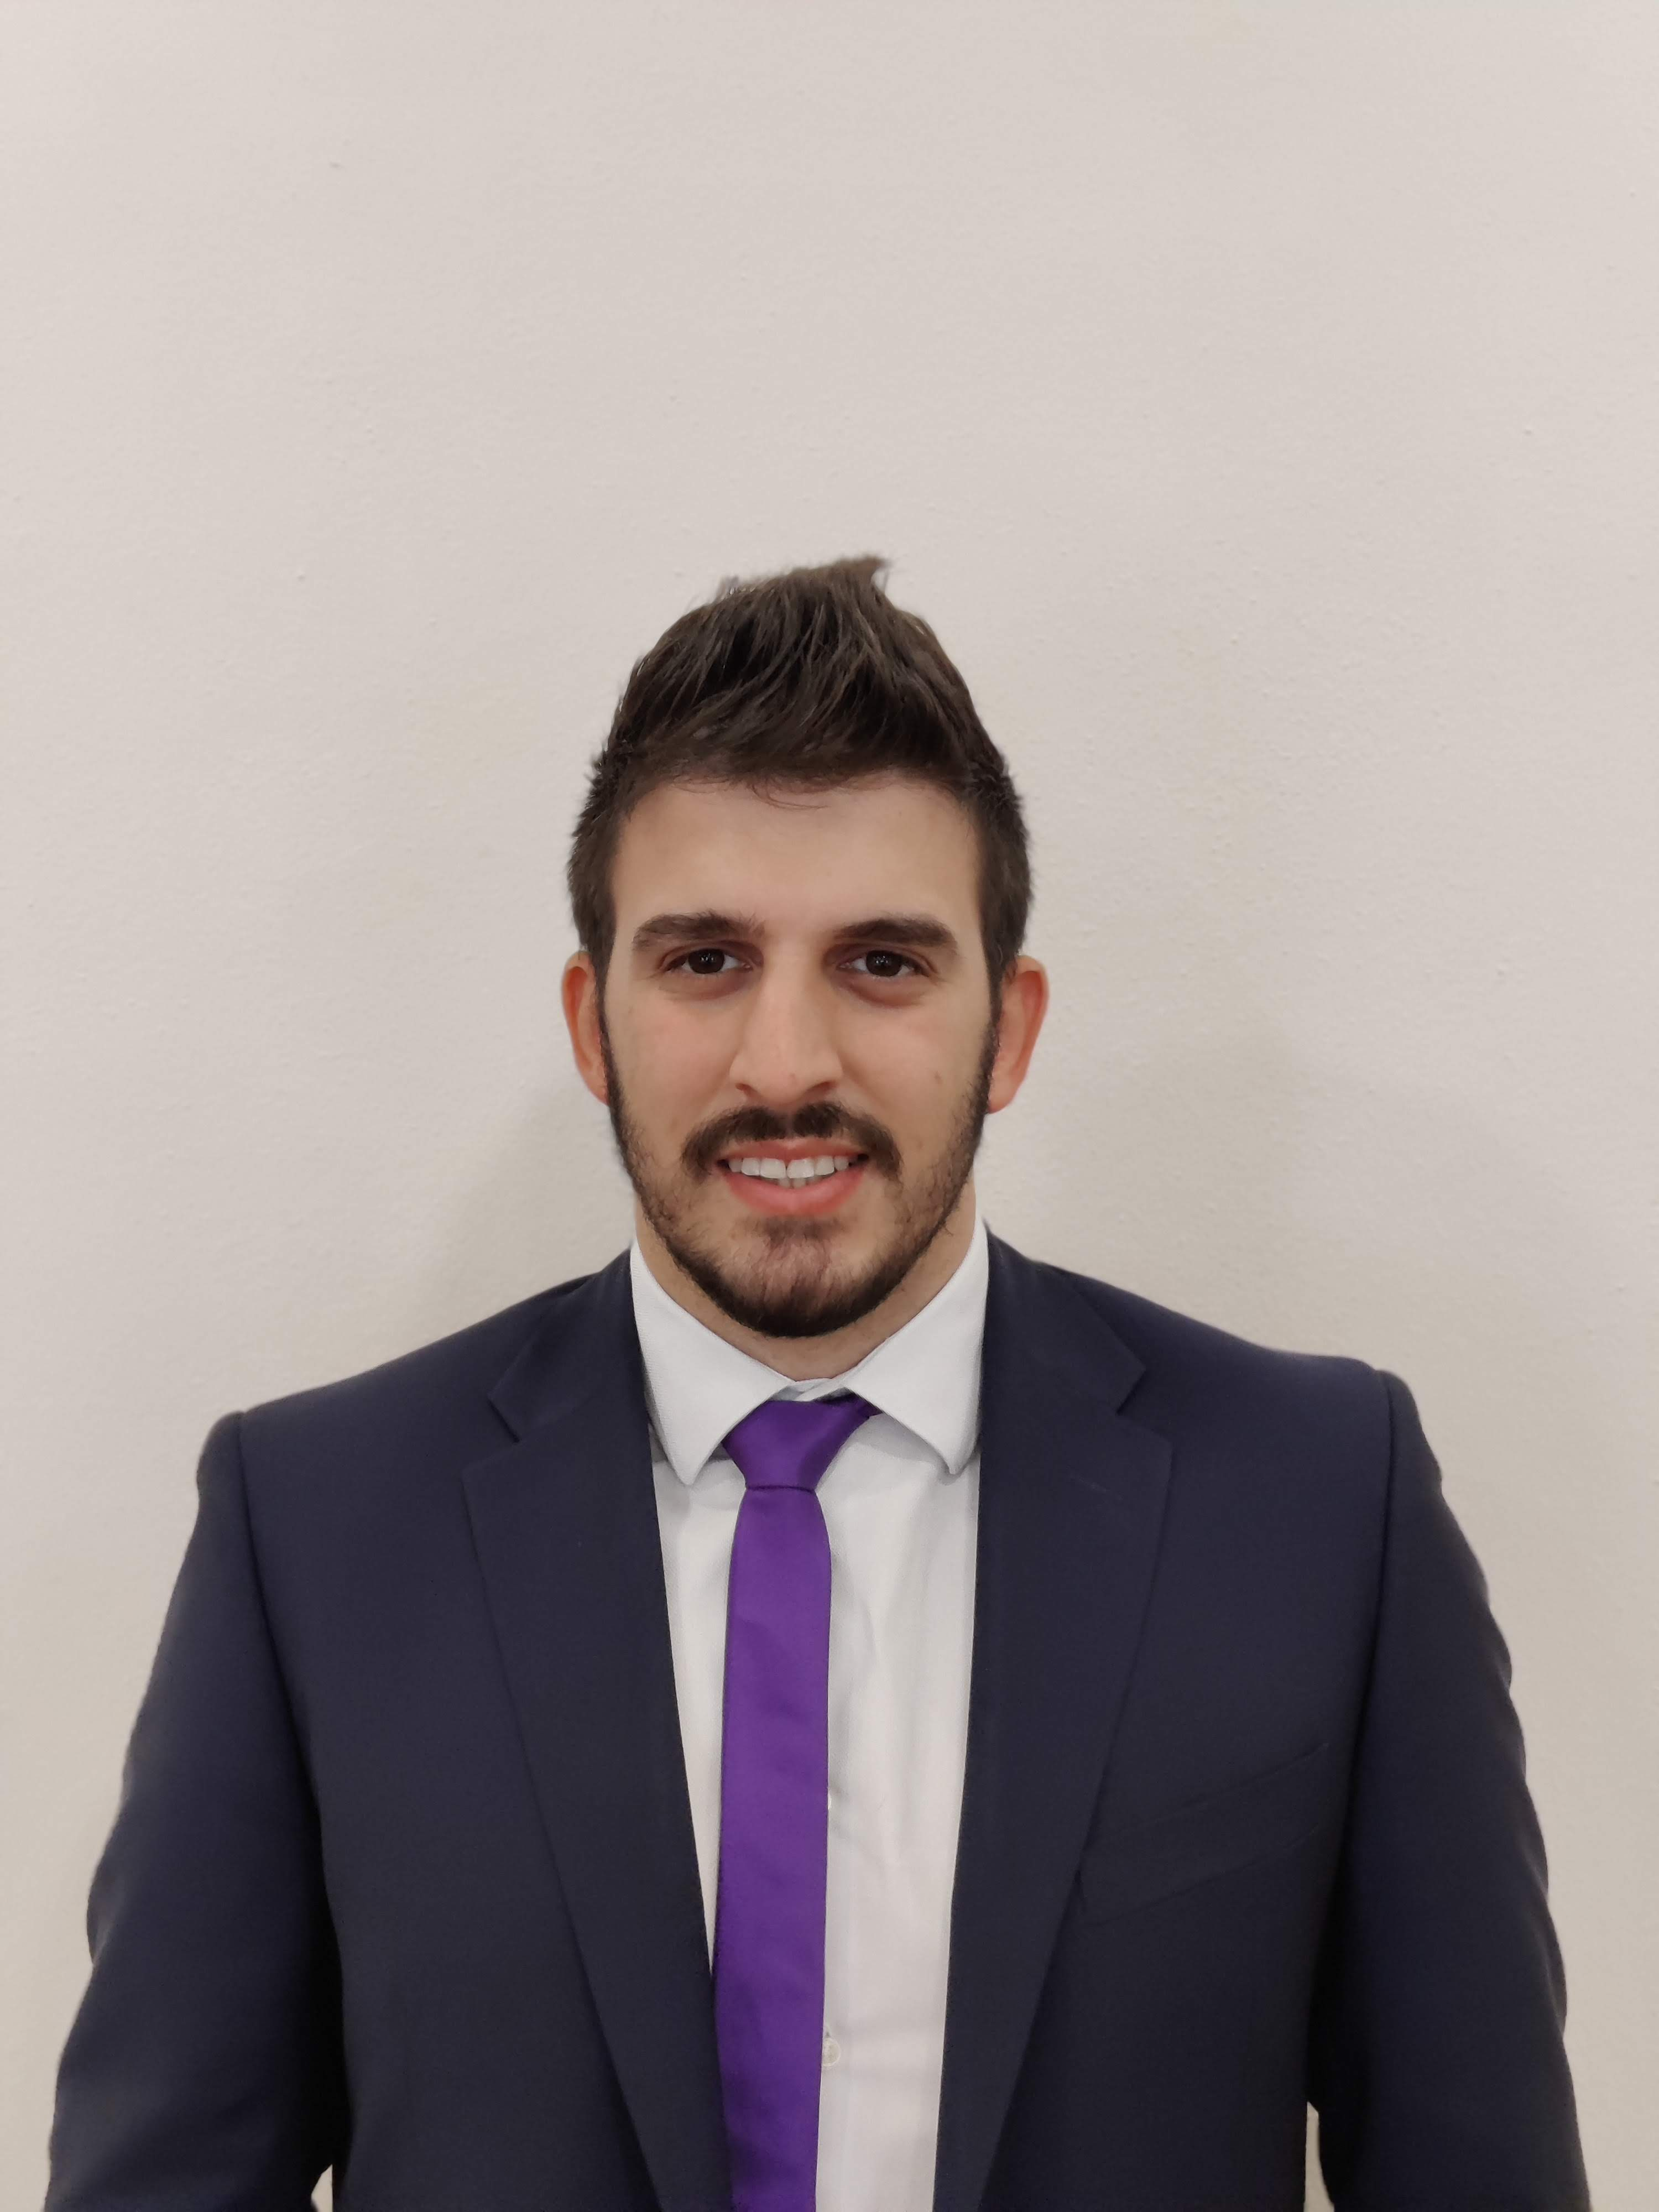
\includegraphics[width=1.0\linewidth]{../shared/Fototessera2.jpg}
	% 
\includegraphics[width=1.0\linewidth]{../shared/Fototessera3.png}
	% 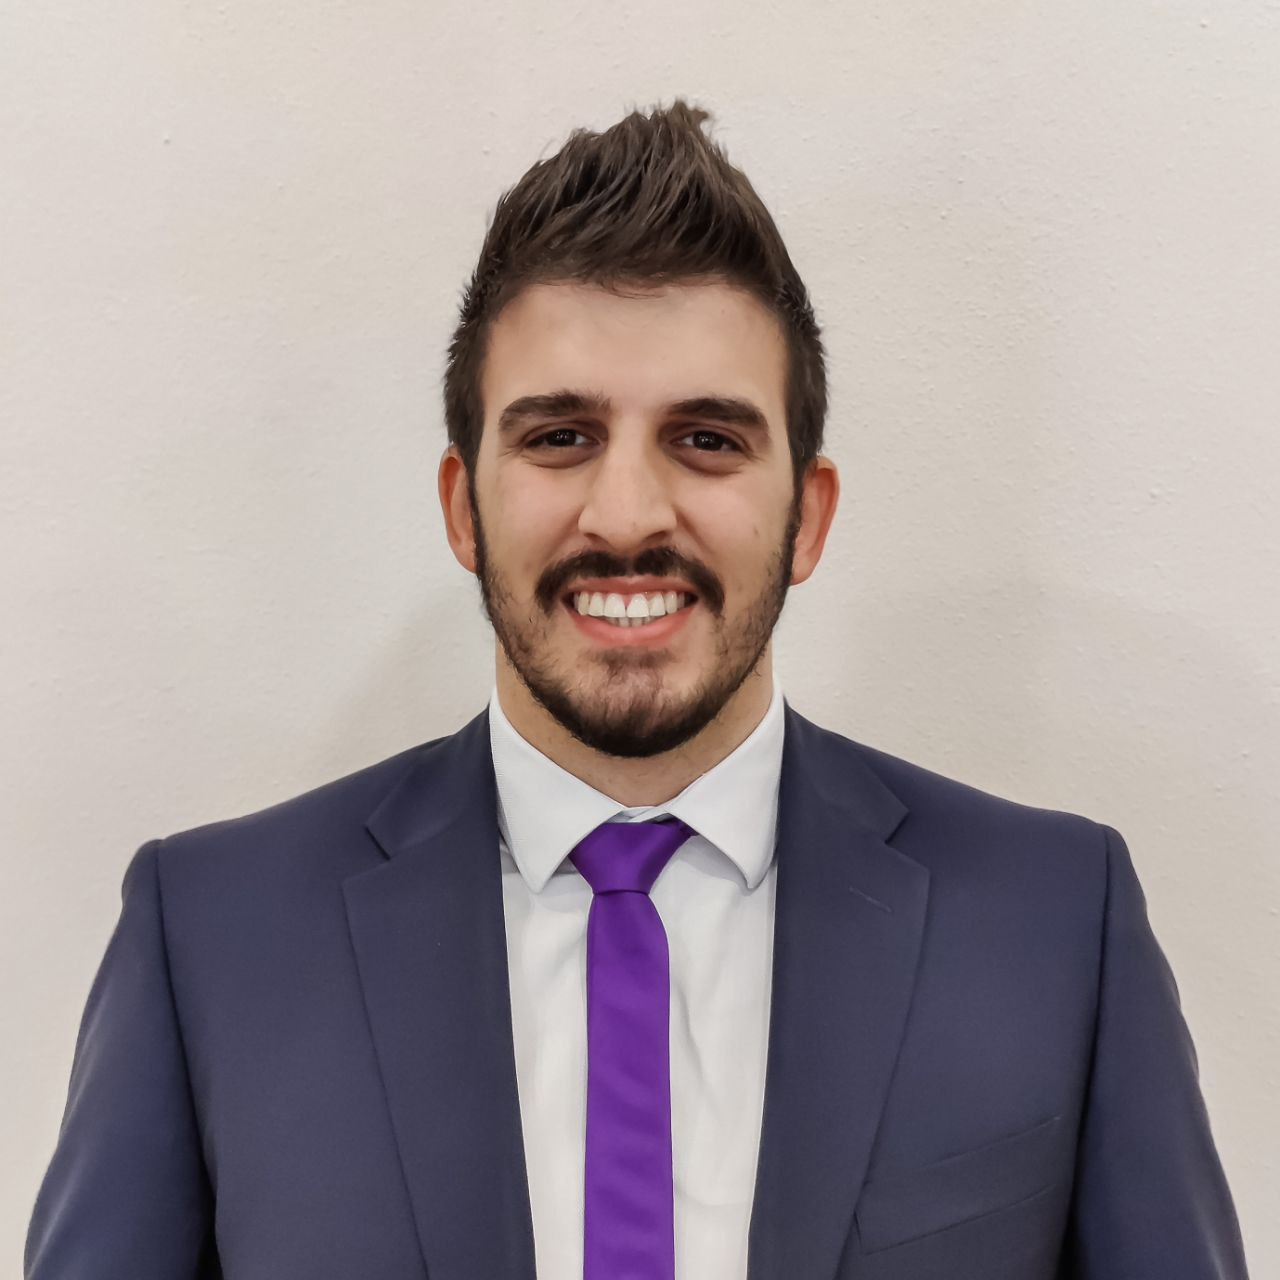
\includegraphics[width=1.0\linewidth]{../shared/Fototessera4.jpg}
	% 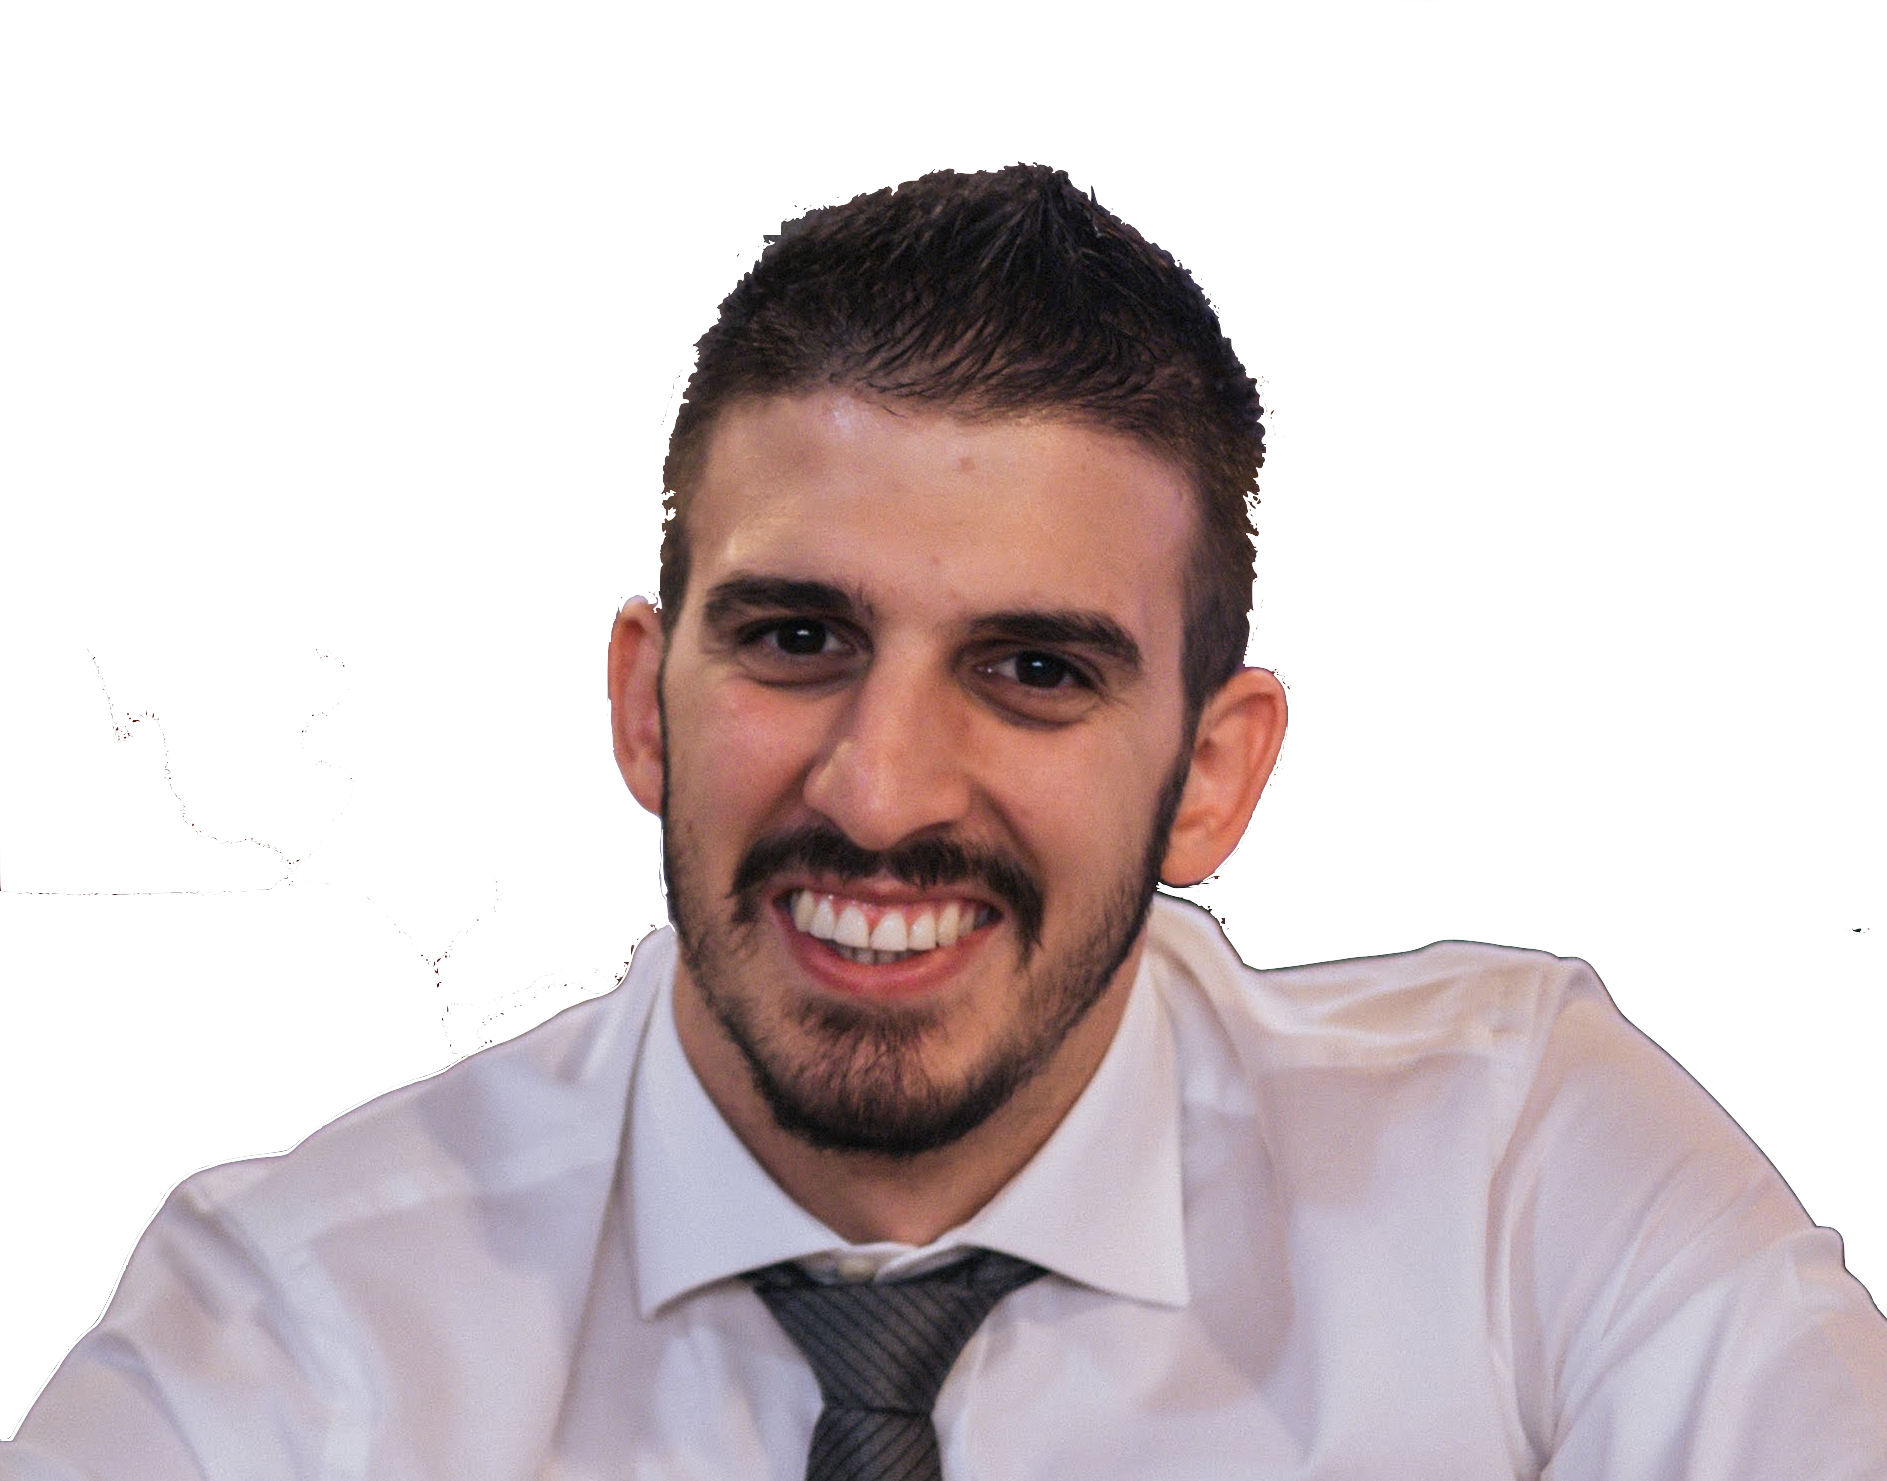
\includegraphics[width=1.0\linewidth]{../shared/test_fototessera.png}
\end{minipage}
%
% \vspace{0.5cm}
%	INTRODUCTION, SKILLS AND TECHNOLOGIES
%
% \cvsect{Who am I?}
%
\begin{minipage}[t]{0.54\textwidth} % 40% of the page width for the introduction text
	\cvsect{Who am I?}
	% \vspace{-\baselineskip} % Required for vertically aligning minipages
%

I am a passionate, pragmatic and goal-driven mechatronics engineer always looking for personal growth opportunities and challenges. This guided my academic choices and allowed me to approach the world of autonomous driving.
To pursue my passion, I became a University researcher and I had the opportunity to work on optimal control problems and algorithms development for ADAS. I collaborated with partners from the automotive and the motorsport industry.
My multidisciplinary education, combined with my interest in practical applications, allows me to address both theoretical and technical aspects of engineering problems.\\
In my work and life, I am always curious, ambitious, open-minded and determined to succeed.
%
\end{minipage}
\hfill % Whitespace between
\begin{minipage}[t]{0.45\textwidth} % 50% of the page for the skills bar chart
	% \vspace{-\baselineskip} % Required for vertically aligning minipages
	\cvsect{Software and programmig skills}
	\begin{barchart}{5.5}
		\baritem{Maple}{100}
		\baritem{Matlab}{80}
		\baritem{C/C++}{80}
		\baritem{LaTeX}{70}
		\baritem{Python}{60}
		\baritem{Mathematica}{40}
		\baritem{CAD}{40}
		\baritem{Ruby}{20}
		\baritem{RTMaps}{20}
		% \baritem{DSPACE}{20}
	\end{barchart}
\end{minipage}
%
% \begin{center}
% 	\bubbles{5/Inventor,3/AutoCAD, 4/ANSYS,3/Visual Studio}
% \end{center}
%
%	EXPERIENCE
%
\cvsect{Working Experiences}
%
\begin{entrylist}
	\entry
		{Sept. 2021-Present}
		{Teaching assistant}
		{University of Trento}
		{Teaching assistant for courses of \textit{"Sistemi Meccanici e Modelli"} e \textit{"Fondamenti di Meccanica"} In collaboration with Prof. Mauro Da Lio and Prof. Emiliano Rustighi.}
	\entry
		{Gen. 2021-Present}
		{Research grant (Decree n. 205/2020)}
		{Università di Trento}
		{Title: "Solution algorithms comparison for minimum-time optimal control problems for racing vehicles"\\
		Supervisor: Prof. Francesco Biral.}
	\entry
		{Jun.-Nov.2020}
		{Research scholarship (Decree n. 74/2020)}
		{University of Trento}
		{Title: “Minimum Time Manoeuvres of complex vehicle models described with DAE".\\ 
		Supervisor: Prof. Francesco Biral.}
	% \entry
	% 	{Sept.--Dec. 2019 \&\\Sept.--Dec. 2018}
	% 	{Tutorship specific areas for mechanics and mechatronics}
	% 	{University of Trento}
	% 	{Frontal lesson, lecture notes and exercises in English for freshmen students of the MSc in Mechatronics Engineering.\\
	% 	Supervisors: Prof. Francesco Biral e Prof. Enrico Bertolazzi.}
	% \entry
	% 	{Apr.--Jun. 2019}
	% 	{Video-lectures for the tutorship of mechanics and mechatronics}
	% 	{University of Trento}
	% 	{Development of video-lectures for the University with topic: linear algebra, scientific calculus, probability/statistics and mechanics.\\
	% 	Supervisors: Prof. Daniele Fontanelli e Prof. Francesco Biral.}

	\entry
		{Apr.\;\;--\,Jun. 2019 \&\\Sept.--Dec. 2019 \&\\Sept.--Dec. 2018}
		{Tutorship specific areas for mechanics and mechatronics and Video-lectures}
		{University of Trento}
		{Frontal lecturer, notes, exercises and video lecture in English for freshmen students of the MSc in Mechatronics Engineering. The videos are available on the Youtube channel of the DII.\\
		Supervisors: Prof. F. Biral, Prof. E. Bertolazzi, Prof. D. Fontanelli, Prof. D. Bortoluzzi}
	\entry
		{Jun.--Sept. 2017\\\footnotesize{Internship}}
		{Internship in Quality Control department}
		{SIAP s.p.a. gruppo CARRARO}
		{Precision measurements of mechanical components, development of sequential charts, specific control plans (SPC), CCP, measurements for capability analysis (Cp, Cpk, \textit{etc.}).
		}
	% \entry
	% 	{Jun.--Sept. 2013 \&\\Jun.--Sept. 2012}
	% 	{Plumber apprentice}
	% 	{DE NARDO ALESSANDRO IMPIANTI TERMOIDRAULICI}
	% 	{Plumber apprentice during summer season.}
\end{entrylist}
%
%
%	PROJECTS
%
\cvsect{Projects Working On}
%
\begin{entrylist}
	\entry
		{Gen. 2021-Present}
		{Minimum Lap Time Simulator}
		{APRILIA RACING \& University of Trento}
		{In collaboration with Aprilia Racing team we develop algorithms to solve optimal control problem for minimum lap time purposes on a complete motorcycle dynamic model. This work is a direct spin-off of my master thesis.}
	\entry
		{Apr. 2022-Present}
		{VeDi 2025}
		{CRF \& University of Trento}
		{Collaboration with CRF (\textit{Fiat Research Centre}) within the european project VeDi 2025. Our contribute is the development of algorithms to plan and negotiate manoeuvres for autonomous vehicles equipped with ADAS systems. }
	\entry
		{May. 2022-Present}
		{Automatic generation of racetracks for vehicle simulators}
		{AnteMotion \& University of Trento}
		{Collaboration with AnteMotion to develop a toolchain for automatic generation of racetracks and scenarios for vehicle simulators. }
\end{entrylist}
%
\pagebreak
%
%	EDUCATION
%
\cvsect{Education}
%
\begin{entrylist}
	\entry
		{Dec. 2020}
		{Professional qualification to practice as an engineer}{University of Trento}{Industrial Engineer}
	\entry
		{2017 -- 2020}
		{Master of Science degree in Mechatronics Engineering}
		{University of Trento}
		{Curriculum mechanics e mechatronics. MSc offered entirely in English.\\
		Main courses: modeling and simulation of mechatronics systems, dynamic and control of vehicles and robots, automatic control, industrial robotics.}
		% computer vision, mechanical vibration,, automatic control
		% \hfill Grade:108/110
	\entry
		{2013 -- 2017}
		{Bachelor of Science degree in Mechanical Engineering}
		{University of Udine}
		{Main courses: thermodynamics and heat transmission, applied mechanics, fluid-dynamics, turbomachinery, mechanics of solids and mechanical design, mechanical technology.} % \hfill Grade:94/110
	\entry
		{2008 -- 2013}
		{Scientific High school diploma}
		{Liceo Scientifico "Michelangelo Grigoletti"}
		{High school diploma with curriculum PNI (National Informatics Plan). } % \hfill Grade:67/100
\end{entrylist}
%
%	ADDITIONAL INFORMATION
%
\begin{minipage}[t]{0.27\textwidth}
	\vspace{-\baselineskip} % Required for vertically aligning minipages
	\cvsect{Languages}
%
	\textbf{Italian} - Native\\
	\textbf{English}  - Fluent, C1 level (IELTS)
%
\end{minipage}
\hfill
\begin{minipage}[t]{0.38\textwidth}
	\vspace{-\baselineskip} % Required for vertically aligning minipages
	%
	\cvsect{Hobbies}
	%
	It might sound oxymoronic, but I am passionate about technology and nature. 
	I build and program small and automated projects with microcontroller and love to spend time in the mountains.
%
\end{minipage}
\hfill
\begin{minipage}[t]{0.27\textwidth}
	\vspace{-\baselineskip} % Required for vertically aligning minipages
	%
	\cvsect{Sports}
%
	I am an amateur climber and I practice both alpine ski and ski touring. I also enjoy football and mountain trail running. 
%
\end{minipage}

% \pagebreak 
\vfill

%----------------------------------------------------------------------------------------



\cvsect{Privacy}

In compliance with the Italian Legislative Decree no. 196 dated 30/06/2003, I hereby authorize the recipient of this document to use and process my personal details for the purpose of recruiting and selecting staff and I confirm to be informed of my rights in accordance to art. 7 of the above mentioned decree.

\vspace{0.5cm}
Trento, \today \\

\vspace{0.2cm}

\includegraphics[width=0.25\textwidth]{../shared/firma.jpg}


\end{document}
